
\documentclass[../Main.tex]{subfiles}
\begin{document}
Based on the real-world problems discussed in Chapter 1, Chapter 2 aims to delve deeper into the existing products and solutions that can help address these issues. Specifically, it will also analyze some detailed use cases of the Data Management System, as outlined in Section 2.2.
\section{Status survey}
\label{section:2.1}
Thông thường, khảo sát chi tiết về hiện trạng và yêu cầu của phần mềm sẽ được lấy từ ba nguồn chính, đó là (i) người dùng/khách hàng, (ii) các hệ thống đã có, (iii) và các ứng dụng tương tự.
Sinh viên cần tiến hành phân tích, so sánh, đánh giá chi tiết ưu nhược điểm của các sản phẩm/nghiên cứu hiện có. Sinh viên có thể lập bảng so sánh nếu cần thiết. Kết hợp với khảo sát người dùng/khách hàng (nếu có), sinh viên nêu và mô tả sơ lược các tính năng phần mềm quan trọng cần phát triển.

\section{Functional Overview}
\label{section:2.2}
% Phần \ref{section:2.2} này có nhiệm vụ tóm tắt các chức năng của phần mềm. Trong phần này, sinh viên lưu ý chỉ mô tả chức năng mức cao (tổng quan) mà không đặc tả chi tiết cho từng chức năng. Đặc tả chi tiết được trình bày trong phần \ref{section:2.3}.

\subsection{General use case diagram}
\label{subsection:2.2.1}
The general use case diagram of Data and EPD Devices Management System is illustrated in Figure 1. As per the diagram, the system involves three main agents, namely The Manager, The Administrator, and the EPD devices. The Manager has the ability to manage EPD devices, data and their own accounts. The Administrator inherits the functions of the Manager and can also manage and test the devices more advanced. On the other hand, the EPD devices act as end-users and receive and display data on the screen. They also interact with the system via MQTT protocol.
\begin{figure}[htbp]
    \centering
    \begin{tikzpicture}
        % Define system boundary
        \umlactor[x=0, y=0]{Administrator}
        \umlactor[x=0, y=-4]{Manager}
        \umlactor[x=11.5, y=0]{EPD Devices}
        
        \begin{umlsystem}[x=4, y=0]{System}
            % Define the use cases
            \umlusecase[x=2, y=0, name=usecase1, fill = white]{Manage personal accounts}
            \umlusecase[x=2, y=-2, name=usecase2, fill = white]{Manage devices}
            \umlusecase[x=2, y=-4, name=usecase3, fill = white]{Manage data}
        \end{umlsystem}
        
        % Draw associations
        \umlassoc{Administrator}{usecase1}
        \umlassoc{Administrator}{usecase2}
        \umlassoc{Manager}{usecase2}
        \umlassoc{Manager}{usecase3}
        \umlassoc{Manager}{usecase1}
        \umlassoc{EPD Devices}{usecase1}
        \umlinherit{Administrator}{Manager} 
        
        \draw (-1.5, 2.5) rectangle (13, -6);
    \end{tikzpicture}
    \caption{General use case diagram of the data management system}
    \label{fig:usecasediagram}
\end{figure}

\subsection{Detailed use case diagram}
\label{subsection:2.2.2}

\subsubsection{Detailed use case of User's Account Management function}

Figure 2 below describes the detailed use case diagram of the User's Account Management function, including the Manager and Administrator. Users can create a new account, log in, and modify personal information.

\begin{figure}[htbp]
    \centering
    \begin{tikzpicture}
        \umlactor[x=0, y=0]{Administrator}
        \umlactor[x=0, y=-4]{Manager}
    
        \begin{umlsystem}[x=4, y=0]{System}
            % Define the use cases
            \umlusecase[x=2, y=0, name=usecase1, fill = white]{Register}
            \umlusecase[x=2, y=-2, name=usecase2, fill = white]{Log in}
            \umlusecase[x=2, y=-4, width=3cm, name=usecase3]{Manage personal information}
        \end{umlsystem}
        
        % Draw associations
        \umlassoc{Manager}{usecase1}
        \umlassoc{Manager}{usecase2}
        \umlassoc{Manager}{usecase3}
        \umlinherit{Administrator}{Manager} 
        
        \draw (-1.5, 2.5) rectangle (13, -6);
    \end{tikzpicture}
    \caption{Detailed use case of User's Account Management function}
    \label{fig:usecasediagram}
\end{figure}

\subsubsection{Detailed use case of Data Management function}
A detailed use case diagram of the Data Management function of the Manager is displayed in Figure 3. This function enables the Manager to view a list of data, add, modify, or remove data information, and choose whether to display the data on the device or not.

\begin{figure}[htbp]
    \centering
    \begin{tikzpicture}
        \umlactor[x=0, y=-2]{Manager}
        \umlactor[x=11.5, y=-1]{EPD Devices}
        
        \begin{umlsystem}[x=4, y=0]{System}
            % Define the use cases
            \umlusecase[x=2, y=0, name=usecase1]{Add displaying data}
            \umlusecase[x=2, y=-2, name=usecase2]{Modify data information}
            \umlusecase[x=2, y=-4, width=3cm, name=usecase3]{Display data on device}
            \umlusecase[x=2, y=-6, width=3cm, name=usecase4]{Remove data}
        \end{umlsystem}
        
        % Draw associations
        \umlassoc{Manager}{usecase1}
        \umlassoc{Manager}{usecase2}
        \umlassoc{Manager}{usecase3}
        \umlassoc{Manager}{usecase4}
        \umlassoc{EPD Devices}{usecase2}
        \umlassoc{EPD Devices}{usecase3}
        
        \draw (-1.5, 2.5) rectangle (13, -8);
    \end{tikzpicture}
    \caption{Detailed use case of Data Management function}
    \label{fig:usecasediagram}
\end{figure}

\subsubsection{Detailed use case of Device Management function}
Figure \ref{} illustrates the use case diagram of the Device Management function, showing 2 actors participating in the system. This function enables the Manager to view a list of devices add, modify, or remove device information. The Administrator, inheriting the functions of the Manager, can also debug the device after connecting it to the computer via a USB port. 

\subsection{Business process}
\label{subsection:2.2.3}
In the system, there are many business processes, the most prominent are the process of adding data and displaying it on EPD devices, and the process of adding EPD devices to the system.  Each flow demonstrates how the system communicates with the device via USB and the MQTT protocol, and how the device receives and processes data.

\subsubsection{"Creating new device" flow}
Figure \ref{} below shows the business process when the Manager creates and registers a new device to the system. This process requires the users to connect the EPD device to the computer via a USB port, choose from the list of connected devices, and then fill in the information before submitting it to the system. After the system receives the submitted data, it sends the data write request to the device via Serial Port. The device will connect to the internet with the information received, and then connect to MQTT Broker before publishing its connection status to the system.

\begin{figure}[H]
    \centering
    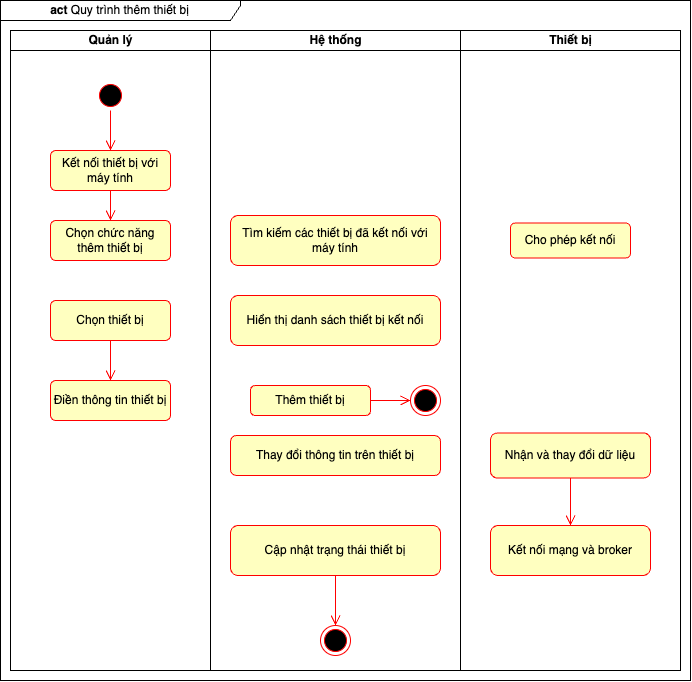
\includegraphics[scale=0.6]{doc/thesis/EN/imgs/act_new-device.png}
    \caption{Quy trình tạo thiết bị mới.}
    \label{fig:uc-general}
\end{figure}
\subsubsection{"Creating and displaying new data" flow}
Figure 6 below describes the business process when users add data to the system. First, the user will select the type of data they want to display, and then, based on the selected data type, the user will add the corresponding detailed information. Users can also choose whether to allow display on the EPD device or not. If allowed, the system will get a list of devices connecting to the MQTT Server for the user to choose from, and the user will fill in additional information about how to display on the device. After receiving information from the user, the system will send MQTT messages via MQTT Broker, and the selected device will receive and display the information and send back the status to the system via MQTT protocol.

\begin{figure}[H]
    \centering
    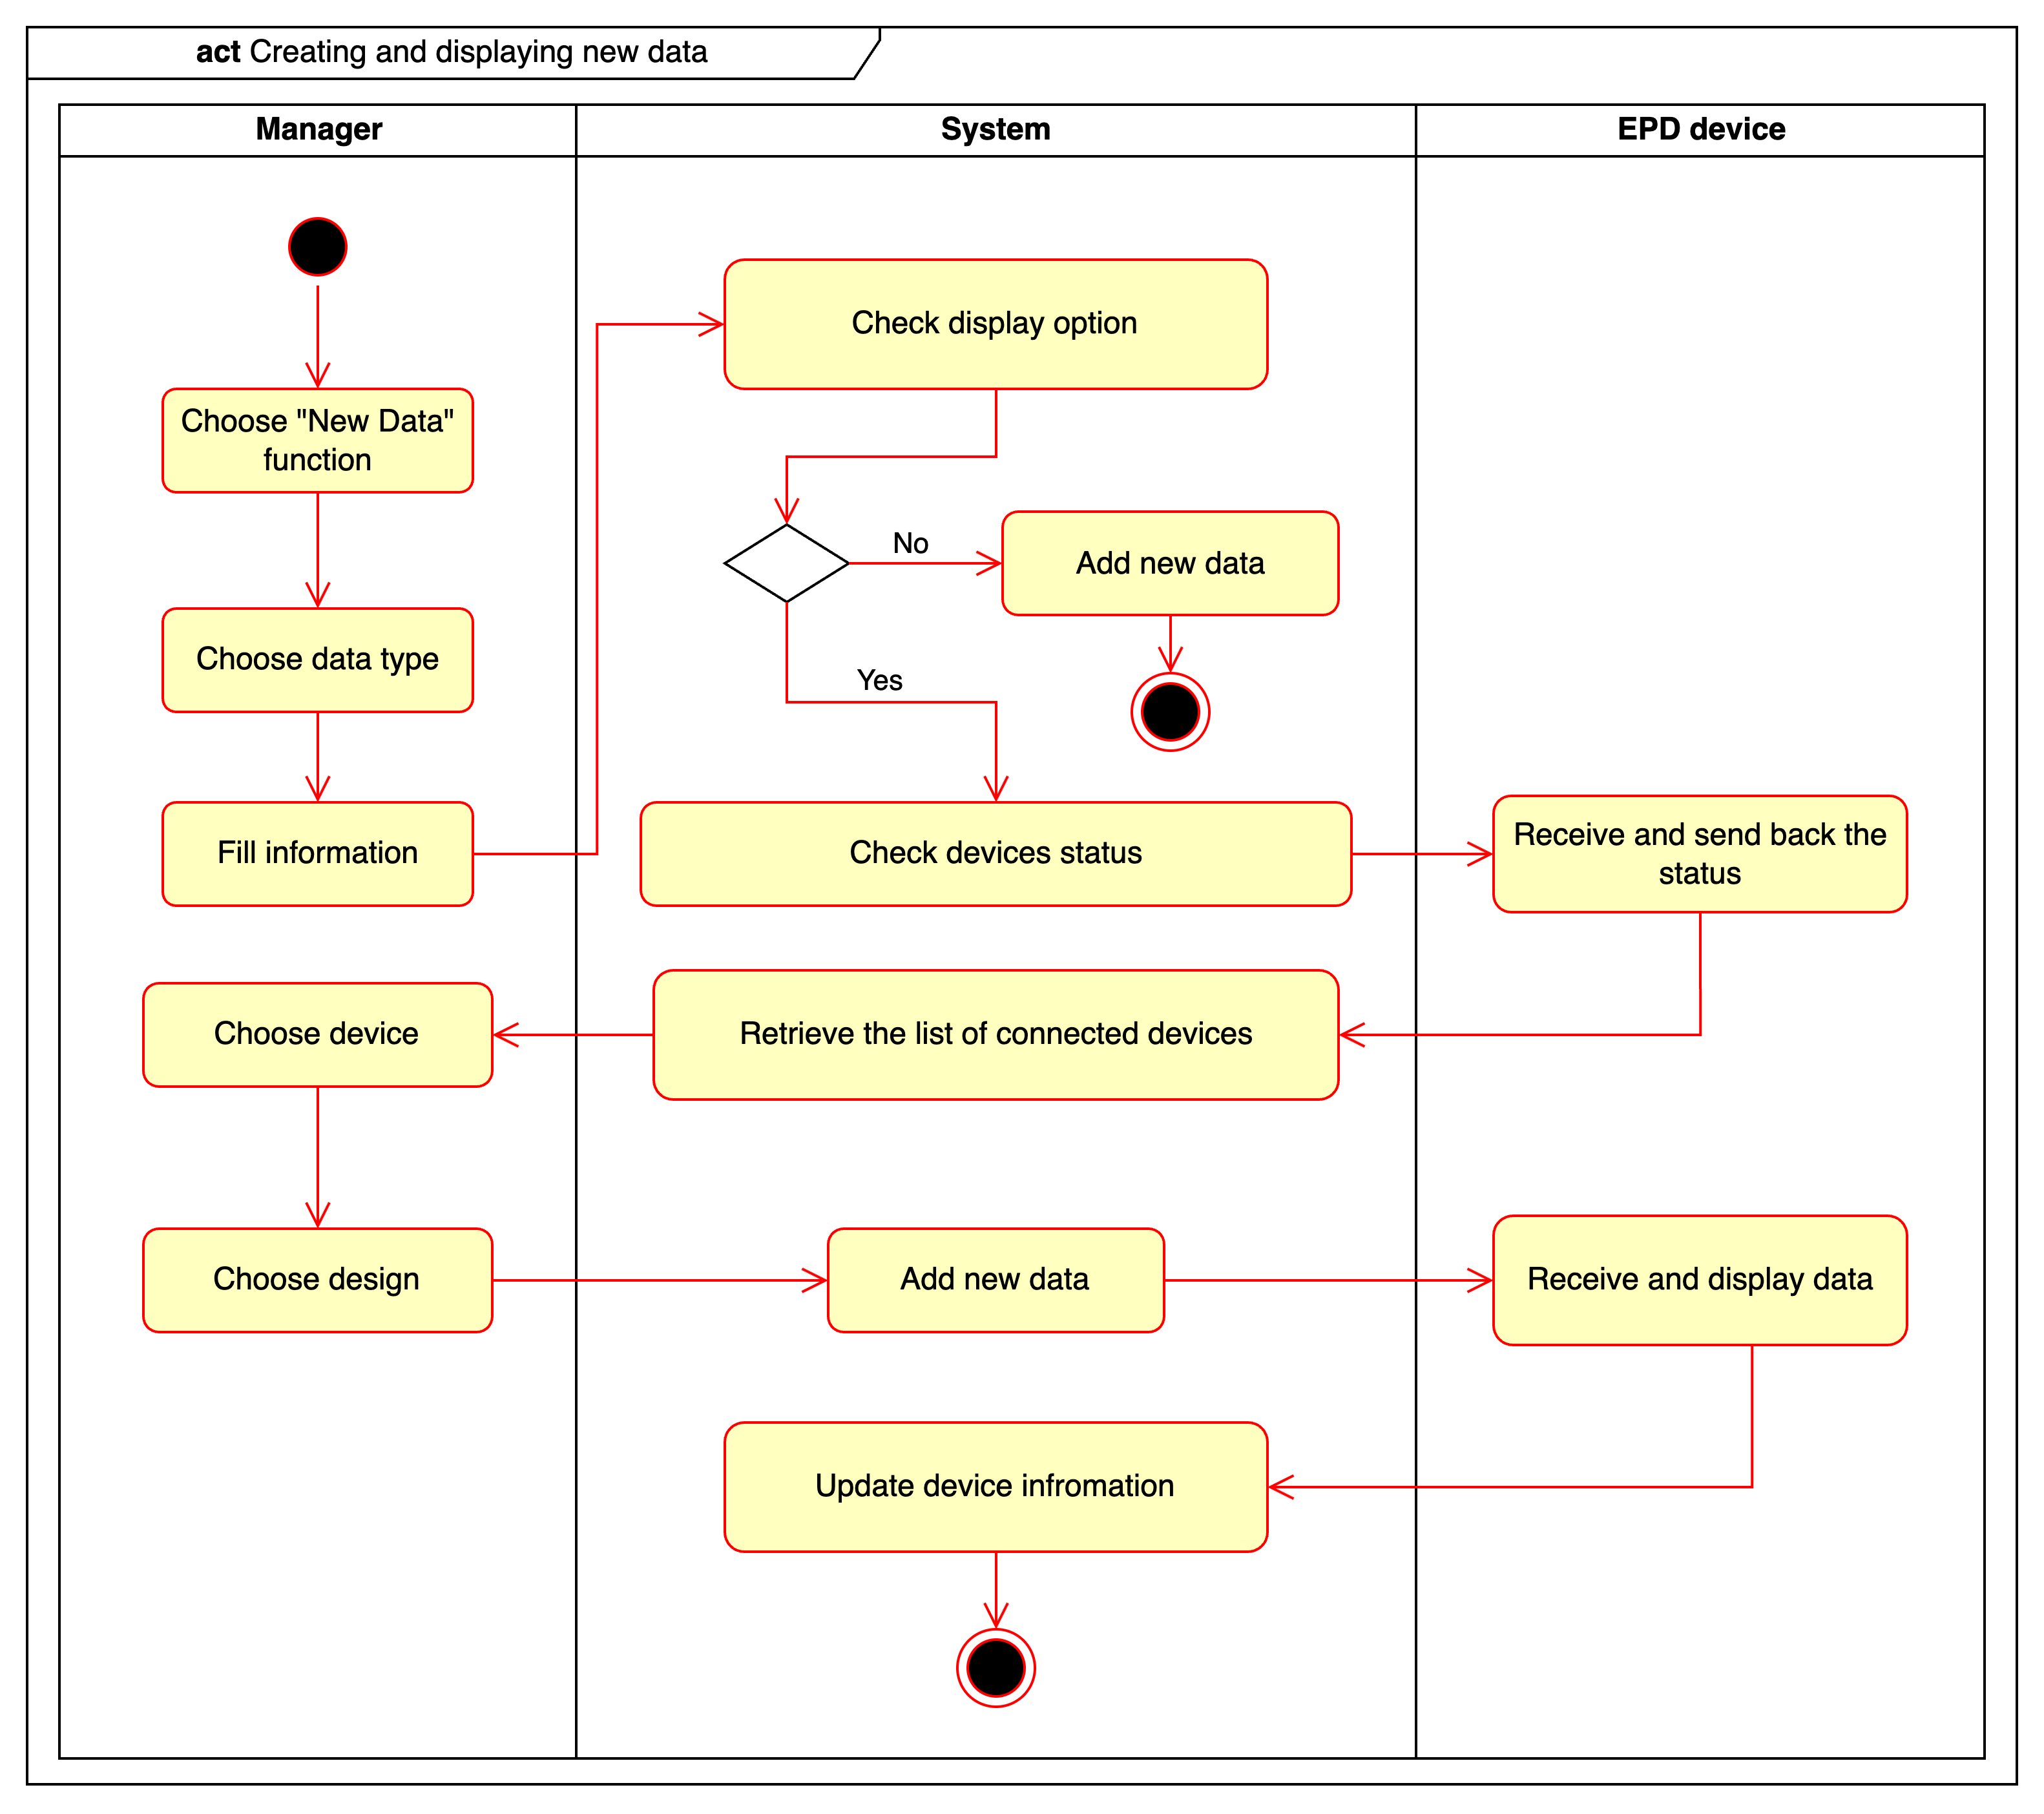
\includegraphics[scale=0.6]{doc/thesis/EN/imgs/act_new-data.png}
    \caption{Quy trình tạo dữ liệu và hiển thị trên thiết bị.}
    \label{fig:uc-general}
\end{figure}

\section{Functional description}
\label{section:2.3}
Sinh viên lựa chọn từ 4 đến 7 use case quan trọng nhất của đồ án để đặc tả chi tiết. Mỗi đặc tả bao gồm ít nhất các thông tin sau: (i) Tên use case, (ii) Luồng sự kiện (chính và phát sinh), (iii) Tiền điều kiện, và (iv) Hậu điều kiện. Sinh viên chỉ vẽ bổ sung biểu đồ hoạt động khi đặc tả use case phức tạp. ok kj ghj

\begin{table}[H]
    \newcolumntype{M}[1]{>{\centering\arraybackslash}m{#1}}
    \newcolumntype{L}[1]{>{\raggedright\arraybackslash}p{#1}}
    \renewcommand{\arraystretch}{2} % Adjust for row height
    \centering{}
    \fontsize{7pt}{8pt}\selectfont 
    \begin{tabular}{| m{2cm} | m{4cm} |}
        \hline
        \textbf{ID} & \textbf{Name}             \\ \hline
        UC01        & Create new device         \\ \hline
        UC02        & Modify device information \\ \hline
        UC03        & Delete device             \\ \hline
        UC04        & Add new data              \\ \hline
        UC05        & Modify data information   \\ \hline
        UC06        & Remove data               \\ \hline
        UC07        & Create account            \\ \hline
        UC08        & Sign in                   \\ \hline
    \end{tabular}
    \caption{Danh sách thư viện và công cụ sử dụng}
    \label{fig:table_tools}
\end{table}

\subsection{Description of use case "Create new device"}
{\fontsize{9pt}{8pt}\selectfont 
    \newcolumntype{M}[1]{>{\centering\arraybackslash}m{#1}}
    \newcolumntype{L}[1]{>{\raggedright\arraybackslash}p{#1}}
    \renewcommand{\arraystretch}{2.5} % Adjust for row height
    \begin{longtable}{|L{2cm}|L{1cm}|L{2cm}|L{7cm}|}
        \hline
        \textbf{ID}             & UC01 & \textbf{Name} & Device Management \\ \hline
        \textbf{Actor}          & \multicolumn{3}{l|}{Manager, EPD device} \\ \hline
        \textbf{Pre-condition}  & \multicolumn{3}{p{12cm}|}{The user logs into the system as a Manager. To create a new device and edit device information in case the device is not connected to the Internet, users need to connect the device to the computer via a USB port.} \\ \hline
        
        \hline
        \multirow{0}{2cm}{\textbf{Main scenario (success)}} & 
        \textbf{No.} & \textbf{Executed by} & \textbf{Action} \\ \cline{2-4}
        \endfirsthead
        \hline
        \multirow{0}{2cm}{\textbf{Main scenario (success)}} & 
        \textbf{No.} & \textbf{Executed by} & \textbf{Action} \\ \cline{2-4}
        \endhead
        & 1     & Manager               & Select "New Device" function\\ \cline{2-4}
        & 2     & System                & Retrieve and display the list of devices connected via USB \\ \cline{2-4}
        & 3     & Manager               & Choose a device from the list \\ \cline{2-4}
        & 4	    & System                & Connect to the device via Serial Port \\ \cline{2-4}
        & 5	    & System	            & Display the interface to enter device information \\ \cline{2-4}
        & 6     & Manager	            & Fill in the device information (described below *) \\ \cline{2-4}
        & 7     & Manager	            & Send a request to create a new device \\ \cline{2-4}
        & 8	    & System	            & Store device information at the server and transmit data to the connected device \\ \cline{2-4}
        & 8.1	& System	            & Store device information at the server \\ \cline{2-4}
        & 8.2	& System	            & Transmit data to the EPD device \\ \cline{2-4}
        & 8.2.1	& Connected EPD device  & Process the received information \\ \cline{2-4}
        & 8.2.2	& Connected EPD device  & Connect to the Internet and MQTT Broker \\ \cline{2-4}
        & 8.2.3	& Connected EPD device	& Send status information to the server \\ \cline{2-4}
        & 8.2.4	& System	            & Receive and edit information of the new device \\ \cline{2-4}
        & 9	    & System	            & Notify successful device creation \\ \hline
    
        \multirow{0}{2cm}{\textbf{Extensions}} & 
        \textbf{No.} & \textbf{Executed by} & \textbf{Action} \\ \cline{2-4}
        & 4a.	 & System	& Error message: unable to connect to the device\\ \cline{2-4}
        & 8.1a	 & System	& Error message: need to enter all required fields of the device if the Manager misses any\\ \cline{2-4}
        & 8.2.2a & System	& If no update response is received from the device, save the device information\\ \hline
    \end{longtable}
}

\subsection{Description of use case "Modify device's information"}
{\fontsize{9pt}{8pt}\selectfont 
    \newcolumntype{M}[1]{>{\centering\arraybackslash}m{#1}}
    \newcolumntype{L}[1]{>{\raggedright\arraybackslash}p{#1}}
    \renewcommand{\arraystretch}{2.5} % Adjust for row height
    \begin{longtable}{|L{2cm}|L{1cm}|L{2cm}|L{7cm}|}
        \hline
        \textbf{ID}             & UC01 & \textbf{Name} & Device Management \\ \hline
        \textbf{Actor}          & \multicolumn{3}{l|}{Manager, EPD device} \\ \hline
        \textbf{Pre-condition}  & \multicolumn{3}{p{12cm}|}{The user logs into the system as a Manager. To create a new device and edit device information in case the device is not connected to the Internet, users need to connect the device to the computer via a USB port.} \\ \hline
        
        \hline
        \multirow{0}{2cm}{\textbf{Main scenario (success)}} & 
        \textbf{No.} & \textbf{Executed by} & \textbf{Action} \\ \cline{2-4}
        \endfirsthead
        \hline
        \multirow{0}{2cm}{\textbf{Main scenario (success)}} & 
        \textbf{No.} & \textbf{Executed by} & \textbf{Action} \\ \cline{2-4}
        \endhead
        & 1     & Manager               & Access Dashboard, select Device \\ \cline{2-4}
        & 2     & System                & Retrieve and display the list of registered devices \\ \cline{2-4}
        & 3     & Manager               & Choose a device from the list and select Edit \\ \cline{2-4}
        & 4     & System                & Check the status of the device \\ \cline{2-4}
        & 4.1   & System                & If the device is not connected to the system, display a message asking the user to connect the device via USB \\ \cline{2-4}
        & 4.2   & Manager               & Connect the device via USB and choose from the list of connected devices \\ \cline{2-4}
        & 5     & System                & Display the interface to enter device information (described below *) \\ \cline{2-4}
        & 6     & Manager               & Fill in and send a request to change device information \\ \cline{2-4}
        & 7     & System                & Save the new updated information \\ \cline{2-4}
        & 7.1   & System                & If the device is connected via USB, transmit data to the connected EPD device \\ \cline{2-4}
        & 7.2   & System                & If the device is connected to the MQTT server, send a request to change information on the device via the MQTT protocol \\ \cline{2-4}
        & 8     & Connected EPD device  & Process the received information \\ \cline{2-4}
        & 8.1   & Connected EPD device  & If the device is connected via USB, connect to the Internet and MQTT Broker \\ \cline{2-4}
        & 9     & Connected EPD device  & Send status information to the server \\ \cline{2-4}
        & 10    & System                & Receive and edit information of the new device \\ \cline{2-4}
        & 11    & System                & Notify successful device information change \\ \hline

    
        \multirow{0}{2cm}{\textbf{Extensions}} & 
        \textbf{No.} & \textbf{Executed by} & \textbf{Action} \\ \cline{2-4}
        & 4.2a.  & System    & Error message: unable to connect to the device \\ \cline{2-4}
        & 7a.    & System    & Error message: need to enter all required fields of the device if Manager misses any \\ \cline{2-4}
        & 10a.   & System    & If no update response is received from the device, save the device information \\ \hline

    \end{longtable}
}

\subsection{Description of use case "Remove a device"}
{\fontsize{9pt}{8pt}\selectfont 
    \newcolumntype{M}[1]{>{\centering\arraybackslash}m{#1}}
    \newcolumntype{L}[1]{>{\raggedright\arraybackslash}p{#1}}
    \renewcommand{\arraystretch}{2.5} % Adjust for row height
    \begin{longtable}{|L{2cm}|L{1cm}|L{2cm}|L{7cm}|}
        \hline
        \textbf{ID}             & UC01 & \textbf{Name} & Device Management \\ \hline
        \textbf{Actor}          & \multicolumn{3}{l|}{Manager, EPD device} \\ \hline
        \textbf{Pre-condition}  & \multicolumn{3}{p{12cm}|}{The user logs into the system as a Manager. To create a new device and edit device information in case the device is not connected to the Internet, users need to connect the device to the computer via a USB port.} \\ \hline
        
        \hline
        \multirow{0}{2cm}{\textbf{Main scenario (success)}} & 
        \textbf{No.} & \textbf{Executed by} & \textbf{Action} \\ \cline{2-4}
        \endfirsthead
        \hline
        \multirow{0}{2cm}{\textbf{Main scenario (success)}} & 
        \textbf{No.} & \textbf{Executed by} & \textbf{Action} \\ \cline{2-4}
        \endhead
        
        & 1     & Manager               & Access the Dashboard, select Device \\ \cline{2-4}
        & 2     & System                & Retrieve and display the list of registered devices \\ \cline{2-4}
        & 3     & Manager               & Choose a device from the list and select Delete \\ \cline{2-4}
        & 4     & System                & Display a warning asking the user to confirm deletion \\ \cline{2-4}
        & 5     & Manager               & Confirm deletion of data \\ \cline{2-4}
        & 6     & System                & Check the display status of the device \\ \cline{2-4}
        & 6.1   & System                & If the device is not displaying data, remove the device from the system \\ \cline{2-4}
        & 6.2   & System                & If the device is displaying data, send a request to delete data on the device via MQTT \\ \cline{2-4}
        & 6.2.1 & Connected EPD Device  & Process the received information, delete the displaying data information \\ \cline{2-4}
        & 6.2.3 & System                & Remove device display information from the data \\ \hline
    
        \multirow{0}{2cm}{\textbf{Extensions}} & 
        \textbf{No.} & \textbf{Executed by} & \textbf{Action} \\ \cline{2-4}
        & 6a.    & System               & End the use case if the user confirms not to delete the device \\ \cline{2-4}
        & 6.2.3a & System               & Error message: unable to delete the device if an error occurs during deletion \\ \hline

    \end{longtable}
}

\subsection{Description of use case "Add new data"}
{\fontsize{9pt}{8pt}\selectfont 
    \newcolumntype{M}[1]{>{\centering\arraybackslash}m{#1}}
    \newcolumntype{L}[1]{>{\raggedright\arraybackslash}p{#1}}
    \renewcommand{\arraystretch}{2.5} % Adjust for row height
    \begin{longtable}{|L{2cm}|L{1cm}|L{2cm}|L{7cm}|}
        \hline
        \textbf{ID}             & UC01 & \textbf{Name} & Add new data \\ \hline
        \textbf{Actor}          & \multicolumn{3}{l|}{Manager, EPD device} \\ \hline
        \textbf{Pre-condition}  & \multicolumn{3}{p{12cm}|}{The user logs into the system as a Manager. To create a new device and edit device information in case the device is not connected to the Internet, users need to connect the device to the computer via a USB port.} \\ \hline
        
        \hline
        \multirow{0}{2cm}{\textbf{Main scenario (success)}} & 
        \textbf{No.} & \textbf{Executed by} & \textbf{Action} \\ \cline{2-4}
        \endfirsthead
        \hline
        \multirow{0}{2cm}{\textbf{Main scenario (success)}} & 
        \textbf{No.} & \textbf{Executed by} & \textbf{Action} \\ \cline{2-4}
        \endhead
        & 1     & Manager               & Select "New Data" function \\ \cline{2-4}
        & 2     & System                & Display the interface to choose data type to add \\ \cline{2-4}
        & 3     & Manager               & Choose the type of data from the list \\ \cline{2-4}
        & 4     & System                & Display the interface to enter data information \\ \cline{2-4}
        & 5     & Manager               & Fill in the data information (described below *) \\ \cline{2-4}
        & 6.1     & System                & If the user chooses to display on a device, show the interface to select device and design \\ \cline{2-4}
        & 6.2     & Manager               & If the user doesn't allow to display the data, send a request to create new data \\ \cline{2-4}
        & 7     & System                & Perform saving the data on the server and transmitting it to the connected device \\ \cline{2-4}
        & 7.1   & System                & Save new device information on the server \\ \cline{2-4}
        & 7.2   & System                & Transmit data to the connected EPD device \\ \cline{2-4}
        & 7.2.1 & Connected EPD Device  & Process the received information \\ \cline{2-4}
        & 7.2.2 & Connected EPD Device  & Connect to the Internet and MQTT Broker \\ \cline{2-4}
        & 7.2.3 & Connected EPD Device  & Send status information to the server \\ \cline{2-4}
        & 7.2.4 & System                & Receive and edit the new device information \\ \cline{2-4}
        & 8     & System                & Notify successful creation of the device \\ \hline


    
        \multirow{0}{2cm}{\textbf{Extensions}} & 
        \textbf{No.} & \textbf{Executed by} & \textbf{Action} \\ \cline{2-4}
        &4.2a.	& Hệ thống	& Thông báo lỗi: không thể kết nối đến thiết bị \\ \cline{2-4}
        &7a.	& Hệ thống	& Thông báo lỗi: cần nhập đủ các trường thông tin cần thiết của thiết bị nếu Người quản lý nhập thiếu \\ \cline{2-4}
        &10a.	& Hệ thống	& Không nhận được phản hồi cập nhật trạng thái từ thiết bị, lưu lại thông tin thiết bị \\ \hline
    \end{longtable}
}
\section{Non-functional requirement}
\label{section:2.4}

Given the unique nature of the system, where a user must manage a vast array of data across numerous devices in an open environment, system security is a top priority when facilitating communication between devices. Additionally, the system requires transparency and user-friendliness for new users, including those with physical impairments. Moreover, to operate reliably in large enterprise environments with numerous devices, users, and data, the system also demands high fault tolerance, ease of inspection, upgrades, and maintenance.
\subsection{Security}
\hfill
\subsection{Security}
\hfill
\subsection{Security}
\hfill
\end{document}